% Chapter 3: Surplus edges
% Contains:
%   Definition of surplus edges
%   Eligible edges for s.e.
%   Calculating the probability of s.e.
%   The proof of (Z_n, N_n) => (W,N)
%   Why the overestimated probability is OK

\chapter{Surplus edges} \label{C: surplus edges}
\fxnote{Update title.}

The goal of this chapter will be to first examine under which circumstances surplus edges can arise during the breadth-first walk,
then finding an expression for the probability of encountering one 
and finally proving the joint convergence of $\rznt$ and the surplus edge counting process to $\Wt$ and some limit process dependent on the realisation of $\Wt$.


\section{Counting surplus edges}
%%%%%%%%%%%%%%%%%%%%%%%%%%%%%%%%%%%%%%%%%%%%%%%%%%%%%%%%%%%%
% SECTION: Counting surplus edges
%%%%%%%%%%%%%%%%%%%%%%%%%%%%%%%%%%%%%%%%%%%%%%%%%%%%%%%%%%%%

We begin by describing a way to analyse the appearance of surplus edges.
In Chapter~\ref{C: bf-walk} we defined the breadth-first walk $Z_n$, 
which counted new connections to previously not connected vertices.
We remind ourselves that a surplus edge in a graph $\Gnt$ appears if,
during the transition of vertices and components by the breadth-first walk,
a vertex forms a new connection to another vertex
which already has opened connections to some explored node.
We associate with $\Gcal$ a counting process $(\nnt(s), 0 \leq s \leq n)$, \label{I: nnt}
with $\nnt(0) = 0$, which increases by $1$ at each appearance of a surplus edge.

\begin{figure}[h]
	\centering
	\scalebox{0.85}{
		\begin{tikzpicture}[level distance = 25mm]
% GRAPH
\tikzstyle{level 1}=[sibling distance=22mm]
\tikzstyle{level 2}=[sibling distance=9mm]
\tikzstyle{level 3}=[sibling distance=4mm]
\node (A) [explored] {$v_1$} [grow=right]
	child { node [discovered] {$v_4$}
		child { node [neutral] {}
			edge from parent [dotted]}
		child { node [neutral] {}
			edge from parent [dotted]}
	}
	child { node [discovered] {$v_3$}
		child { node [neutral] {}
			edge from parent [dotted]}
		child { node [neutral] {}
			edge from parent [dotted]}
		child { node [neutral] {}
			edge from parent [dotted]}
	}
	child { node [explored] {$v_2$}
		child { node [discovered] {$v_6$}
			child { node [neutral] {}
				edge from parent [dotted]}
			child { node [neutral] {}
				edge from parent [dotted]}}
		child { node [discovered] {$v_5$}
			child { node [neutral] {}
				edge from parent [dotted]}}
	}
;
% LEGEND NODES
\node [explored, anchor=east](Legend-E-Node) at (10,2.5){};  
\node[anchor=west](Legend-E-Text) at (10,2.5){Explored}; 
\node [discovered, anchor=east](Legend-D-Node) at (10,1.5){};  
\node[anchor=west](Legend-D-Text) at (10,1.5){Discovered}; 
\node [neutrallegend, anchor=east](Legend-N-Node) at (9.9,0.5){};  
\node[anchor=west](Legend-N-Text) at (10,0.5){Neutral}; 
\fxnote{Fix node sizes}
% LEGEND LINES
\draw (9.6,-1) -- (10.05,-1); 
\node[anchor=west](Legend-F-Text) at (10,-1){Edge opened}; 
\draw [dotted] (9.6,-2) -- (10.05,-2); 
\node[anchor=west](Legend-NF-Text) at (10,-2){Edge not yet opened}; 
% LEGEND BOX
\node[draw, fit=(Legend-E-Node)(Legend-N-Text)(Legend-D-Text)(Legend-NF-Text)] {};
\end{tikzpicture}
	}
	\caption{A sample component} 
	\label{F: Surplus Edges Tree}
\end{figure}

To find an expression for the number of vertices which are able to open such excess connections, 
consider the breadth-first walk on the graph of Figure~\ref{F: Surplus Edges Tree} at time $s=2$.
The children of $v_1$, $v_2$ to $v_4$, and the children of $v_2$, that is $v_5$ and $v_6$, are already discovered.
We are interested in surplus edges to $v_3$.
Since $v_1$ to $v_6$ are unable to form edges to become children of $v_3$, we have $\Ineligible{2} = |\{ v_1, \dots,  v_6\}|$.
Of these vertices, $v_1$ and $v_2$ are already explored and every connection to neighbouring nodes is known.
Vertex $v_3$ can not have an edge to itself, so only $v_4$, $v_5$ and $v_6$ are eligible to receive a surplus edge to $v_3$.

Let us examine what these considerations mean in terms of the breadth-first walk $\znt$.
When starting at a new component there are no vertices eligible for a surplus edge.
For each new vertex found as a member of this component we have one additional eligible node 
and with each step taken, one more vertex is explored and thus can no longer receive a surplus edge.
The number of vertices eligible for an excess edge therefore corresponds to the level of the breadth-first walk above its past minimum,
which is attained at the beginning of the component.
Hence we will expect the probability of encountering an excess edge at time $s$ to be proportionate to
\begin{equation} \label{D: zminz}
\zminz(s) := \znt(s) - \min_{u \leq s}\znt(u).
\end{equation}
Rescaling the counting process appropriately this probability should scale to
\begin{equation}
\rzminz(s) := \rznt(s) - \min_{u \leq s}\rznt(u),
\end{equation}
which converges in distribution to
\begin{equation}
\Bt(s) := \Wt(s) - \min_{u \leq s}\Wt(u). 
\end{equation}

In chapter~\ref{C: bf-walk} we examined a similar process, $\Bn$, 
which increased by one for each appearance of a new edge to a previously not connected vertex.
Lemma~\ref{L: formula an} established that $\Bn(s) = \int_{0}^{s} \an(u)du$ with
\begin{equation*}
	\an(s) = (n - \Ineligible{s}) \ps,
\end{equation*}
where $\Ineligible{s}$ is the number of vertices ineligible to become a child of $v_{\ceil{s}}$ at time $s$.
In terms of counting processes, we call $\an$ the rate or conditional intensity of $\Bn$.
It is evident that $\nnt$ will have a similar rate,
substituting the number of vertices eligible to become a child of $v_{\ceil{s}}$ with the number of vertices eligible to receive a surplus edge to $v_{\ceil{s}}$.

In general, at time $i-1$, the first $i$ vertices are ineligible for a surplus edge to $v_i$.
The remaining $\Ineligible{i-1} - i$ vertices are candidates for an excess edge opening with probability $\p$.
Therefore, the counting process $\nnt$ has rate
\begin{equation} \label{E: rate Nnt}
\lambda(s) = (\Ineligible{\floor{s}} - \floor{s}) \ps.
\end{equation}
Note that this rate is only exact for the chance of encountering exactly one surplus edge, 
but an overestimation for multiple excess edges.
If we encounter a surplus edge at some time $s \in [i-1, i)$,
the number of eligible vertices should decrease by one.
However, the number of ineligible vertices in \eqref{E: rate Nnt} is constant for all $s \in [i-1, i)$.
For ease of computation we will continue with this overestimation and later argue that the difference becomes negligible as $n \rightarrow \infty$.

Lemma~\ref{L: formula an} established $\Ineligible{s} = s + \Zetan{\ceil{s}} + \Zn(s)$ 
and using \eqref{E: zeta-1(i) = 1 - min(j)} we can rewrite
\begin{equation*}
\begin{aligned}
\Ineligible{\floor{s}} - \floor{s} 
&= \floor{s} - \ZetaMinus{\floor{s}+1} + \znt(\floor{s}) - \floor{s} \\
&= 1 - \min_{u \leq \floor{s}} \znt(u) + \znt(\floor{s}),
\end{aligned}
\end{equation*}
and the conditional intensity becomes
\begin{equation} \label{E: rate Nnt 2}
\lambda(s) = (1 - \min_{u \leq \floor{s}} \znt(u) + \znt(\floor{s}) \ps.
\end{equation}
We now rescale the counting process via
\begin{equation} \label{E: rescale Nnt}
\rnnt(s) = \nnt(\n{2}{3}s).
\end{equation}
We calculate the rate of this rescaled process.
Recall that the conditional intensity $\bar{\lambda}(s)$ of the process $\rnnt(s)$ must satisfy
\begin{equation}
\Exp{\rnnt(s)} = \int_{0}^{s} \bar{\lambda}(u) du.
\end{equation}
Using \eqref{E: rescale Nnt} we evaluate the above integral in terms of $\lambda(s)$:
\begin{equation*}
\begin{aligned}
\Exp{\rnnt(s)}
&= \Exp{\nnt(\n{2}{3}s)} \\
&= \int_{0}^{\n{2}{3}s} \lambda(u) du \\
&= \int_{0}^{s} \n{2}{3} \lambda(\n{2}{3}u) du.
\end{aligned}
\end{equation*}
Comparing both integrands gives us
\begin{equation} \label{E: conditional intensity final}
\begin{aligned}
\bar{\lambda}(s)
&= \n{2}{3} \lambda(\n{2}{3}s) \\
&= \n{2}{3} \frac{1 - \min_{u \leq \n{2}{3}s} \znt(u) + \znt(\n{2}{3}s)}{1 - (\n{2}{3}s - \floor{\n{2}{3}s})\p} \p \\
&= \n{2}{3} \frac{1 - \n{1}{3} \min_{u \leq s} \rznt(u) + \n{1}{3}\rznt(s)}{1 - (\n{2}{3}s - \floor{\n{2}{3}s})\p} \p \\
&= n \p \frac{\n{-1}{3} - \min_{u \leq s} \rznt(u) + \rznt(s)}{1 - (\n{2}{3}s - \floor{\n{2}{3}s})\p}
\end{aligned}
\end{equation}

Since $n\p \rightarrow 1$ and $|\n{2}{3}s - \floor{\n{2}{3}s}| < 1$ for all $s$ and $n$,
this rate becomes asymptotically close to $\rznt(s) - \min_{u \leq s}\rznt(u)$ as $n \rightarrow \infty$.

By Theorem~\ref{T: Z -> W} we have $\rznt \rightarrow_d \Wt$,
so
\begin{equation}
\bar{\lambda}(s) \rightarrow_d \Wt(s) - \min_{u \leq s}\Wt(u) = \Bt(s).
\end{equation}
The rate of the counting process $\rnnt$ therefore converges in distribution to $\Bt$.

\begin{figure}[ht]
	\centering
	\begin{tikzpicture}
\pgfplotsset{ticks=none}

\begin{axis}[
xmin=0,
axis lines = middle,
xmax=4.2,
ymax = 3.5,
ymin  = 0,
minor xtick = {2.1, 3.3},
width = 10cm,
height = 6.5cm,
clip=false
]

%%%%%%%%%%%%%%%%%%%%%%%%%%%%%%%%%%%%%%%%%%%%%%%%%%%%%%%%%%%%%%%%%%%%%%%%%%%%%%%%
% BROWNIAN MOTION
%%%%%%%%%%%%%%%%%%%%%%%%%%%%%%%%%%%%%%%%%%%%%%%%%%%%%%%%%%%%%%%%%%%%%%%%%%%%%%%%
\addplot [name path=bm1, line width=0.2pt]coordinates{(0,0) (0.0125,0) (0.025,0) (0.0375,0) (0.05,0) (0.0625,0.06) (0.075,0.123) (0.0875,0) (0.1,0.06) (0.1125,0.2) (0.125,0.309) (0.1375,0.251) (0.15,0.539) (0.1625,0.613) (0.175,0.495) (0.1875,0.074) (0.2,0.288) (0.2125,0.279) (0.225,0.276) (0.2375,0.455) (0.25,0.611) (0.2625,0.724) (0.275,0.899) (0.2875,1.048) (0.3,1.062) (0.3125,0.684) (0.325,0.801) (0.3375,0.791) (0.35,0.761) (0.3625,0.482) (0.375,0.391) (0.3875,0.47) (0.4,0.728) (0.4125,0.709) (0.425,0.783) (0.4375,0.772) (0.45,0.511) (0.4625,0.432) (0.475,0.357) (0.4875,0.346) (0.5,0.555) (0.5125,0.7) (0.525,0.668) (0.5375,0.62) (0.55,0.753) (0.5625,0.858) (0.575,0.728) (0.5875,0.593) (0.6,0.662) (0.6125,0.808) (0.625,0.787) (0.6375,0.955) (0.65,1.03) (0.6625,0.914) (0.675,0.979) (0.6875,0.764) (0.7,1.036) (0.7125,1.413) (0.725,1.343) (0.7375,1.145) (0.75,1.253) (0.7625,1.227) (0.775,1.684) (0.7875,1.676) (0.8,1.807) (0.8125,1.813) (0.825,1.671) (0.8375,1.707) (0.85,1.364) (0.8625,1.643) (0.875,1.672) (0.8875,2.085) (0.9,2.175) (0.9125,2.04) (0.925,2.156) (0.9375,1.979) (0.95,1.741) (0.9625,1.796) (0.975,1.712) (0.9875,1.712) (1,1.726) (1.0125,1.614) (1.025,1.506) (1.0375,1.48) (1.05,1.704) (1.0625,1.415) (1.075,1.527) (1.0875,1.591) (1.1,1.793) (1.1125,1.735) (1.125,1.805) (1.1375,1.856) (1.15,1.753) (1.1625,1.983) (1.175,2.203) (1.1875,2.336) (1.2,2.638) (1.2125,2.744) (1.225,2.501) (1.2375,2.392) (1.25,2.16) (1.2625,2.07) (1.275,1.952) (1.2875,1.96) (1.3,1.787) (1.3125,1.817) (1.325,1.692) (1.3375,2.028) (1.35,2.164) (1.3625,2.337) (1.375,2.41) (1.3875,2.73) (1.4,2.609) (1.4125,2.521) (1.425,2.794) (1.4375,2.67) (1.45,2.631) (1.4625,2.556) (1.475,2.495) (1.4875,2.442) (1.5,2.536) (1.5125,2.502) (1.525,2.406) (1.5375,2.661) (1.55,2.621) (1.5625,2.586) (1.575,2.567) (1.5875,2.703) (1.6,2.689) (1.6125,2.682) (1.625,2.552) (1.6375,2.491) (1.65,2.502) (1.6625,2.39) (1.675,2.491) (1.6875,2.202) (1.7,2.261) (1.7125,1.969) (1.725,1.912) (1.7375,1.811) (1.75,1.687) (1.7625,1.676) (1.775,1.312) (1.7875,1.536) (1.8,1.22) (1.8125,1.132) (1.825,0.919) (1.8375,0.777) (1.85,1.173) (1.8625,1.177) (1.875,0.932) (1.8875,0.62) (1.9,0.706) (1.9125,0.703) (1.925,0.642) (1.9375,0.465) (1.95,0.183) (1.9625,0) (1.975,0.168) (1.9875,0.05) (2,0) (2.0125,0.142) (2.025,0.223) (2.0375,0.178) (2.05,0.379) (2.0625,0.548) (2.075,0.43) (2.0875,0.849) (2.1,0.801)
};
\addplot [name path=bm2, line width=0.2pt]coordinates{(2.1,0.801) (2.1125,0.53) (2.125,0.503) (2.1375,0.542) (2.15,0.981) (2.1625,1.001) (2.175,1.088) (2.1875,1.073) (2.2,1.009) (2.2125,1.003) (2.225,1.153) (2.2375,1.547) (2.25,1.742) (2.2625,1.972) (2.275,1.738) (2.2875,1.925) (2.3,1.967) (2.3125,1.688) (2.325,1.787) (2.3375,1.757) (2.35,2.035) (2.3625,1.889) (2.375,1.808) (2.3875,1.632) (2.4,1.598) (2.4125,1.674) (2.425,1.535) (2.4375,1.693) (2.45,1.463) (2.4625,1.264) (2.475,1.538) (2.4875,1.345) (2.5,1.423) (2.5125,1.351) (2.525,1.429) (2.5375,1.75) (2.55,2.051) (2.5625,1.988) (2.575,1.554) (2.5875,2.029) (2.6,2.156) (2.6125,2.258) (2.625,2.256) (2.6375,2.353) (2.65,2.322) (2.6625,2.402) (2.675,2.326) (2.6875,2.065) (2.7,2.253) (2.7125,2.542) (2.725,2.483) (2.7375,2.245) (2.75,2.367) (2.7625,2.358) (2.775,2.029) (2.7875,2.029) (2.8,1.91) (2.8125,1.845) (2.825,1.625) (2.8375,1.968) (2.85,1.905) (2.8625,1.6) (2.875,1.637) (2.8875,1.687) (2.9,1.5) (2.9125,0.951) (2.925,0.829) (2.9375,0.937) (2.95,0.926) (2.9625,0.907) (2.975,1.014) (2.9875,0.788) (3,0.997) (3.0125,0.996) (3.025,1.13) (3.0375,1.327) (3.05,1.369) (3.0625,1.202) (3.075,1.423) (3.0875,1.043) (3.1,0.94) (3.1125,0.891) (3.125,0.859) (3.1375,1.053) (3.15,1.079) (3.1625,1.157) (3.175,1.143) (3.1875,1.096) (3.2,1.229) (3.2125,1.446) (3.225,0.99) (3.2375,1.099) (3.25,1.17) (3.2625,1.089) (3.275,1.27) (3.2875,1.196) (3.3,1.142) 
};
\addplot [name path=bm3, line width=0.2pt]coordinates{(3.3,1.142) (3.3125,1.305) (3.325,1.631) (3.3375,1.683) (3.35,1.603) (3.3625,1.377) (3.375,1.314) (3.3875,1.135) (3.4,1.086) (3.4125,1.161) (3.425,0.999) (3.4375,1.502) (3.45,1.532) (3.4625,1.747) (3.475,1.312) (3.4875,1.453) (3.5,1.202) (3.5125,1.377) (3.525,1.453) (3.5375,1.375) (3.55,1.627) (3.5625,1.494) (3.575,1.384) (3.5875,1.193) (3.6,1.066) (3.6125,1.246) (3.625,1.328) (3.6375,1.519) (3.65,1.445) (3.6625,1.517) (3.675,1.563) (3.6875,1.292) (3.7,1.63) (3.7125,1.656) (3.725,1.801) (3.7375,1.983) (3.75,1.973) (3.7625,1.915) (3.775,2.085) (3.7875,1.886) (3.8,2.26) (3.8125,2.188) (3.825,2.502) (3.8375,2.789) (3.85,2.805) (3.8625,2.913) (3.875,2.718) (3.8875,2.78) (3.9,2.978) (3.9125,2.997) (3.925,2.91) (3.9375,2.786) (3.95,2.779) (3.9625,2.982) (3.975,2.89) (3.9875,2.867) (4,2.621) (4.0125,2.715) (4.025,2.964) (4.0375,3.248) (4.05,3.403) (4.0625,3.048) (4.075,3.139) (4.0875,3.226) (4.1,3.159)
};

%%%%%%%%%%%%%%%%%%%%%%%%%%%%%%%%%%%%%%%%%%%%%%%%%%%%%%%%%%%%%%%%%%%%%%%%%%%%%%%%
% FILL AREA
%%%%%%%%%%%%%%%%%%%%%%%%%%%%%%%%%%%%%%%%%%%%%%%%%%%%%%%%%%%%%%%%%%%%%%%%%%%%%%%%
\path[name path=axis] (axis cs:2.1,0) -- (axis cs:3.3,0);

\addplot [
thick,
color=gray,
fill=gray, 
fill opacity=0.1
]
fill between[
of=bm2 and axis,
%soft clip={domain=0:1},
];


%%%%%%%%%%%%%%%%%%%%%%%%%%%%%%%%%%%%%%%%%%%%%%%%%%%%%%%%%%%%%%%%%%%%%%%%%%%%%%%%
% THICK LINES
%%%%%%%%%%%%%%%%%%%%%%%%%%%%%%%%%%%%%%%%%%%%%%%%%%%%%%%%%%%%%%%%%%%%%%%%%%%%%%%%

\addplot [name path=int, line width=1pt]coordinates{(2.1,0) (3.3,0)};

\draw [decorate,decoration={brace,amplitude=5pt,raise=4pt, mirror},yshift=0pt]
(axis cs: 2.1,0) -- (axis cs: 3.3,0) node [black,midway, anchor = north, yshift = -0.3cm] {\footnotesize
	$I$};

%%%%%%%%%%%%%%%%%%%%%%%%%%%%%%%%%%%%%%%%%%%%%%%%%%%%%%%%%%%%%%%%%%%%%%%%%%%%%%%%
% MARKS / LABELS
%%%%%%%%%%%%%%%%%%%%%%%%%%%%%%%%%%%%%%%%%%%%%%%%%%%%%%%%%%%%%%%%%%%%%%%%%%%%%%%%

\node[font=\fontsize{15}{15}\selectfont] at (axis cs:0.288,0) {$\times$};
\node[font=\fontsize{15}{15}\selectfont] at (axis cs:0.654,0) {$\times$};
\node[font=\fontsize{15}{15}\selectfont] at (axis cs:1.2,0) {$\times$};
\node[font=\fontsize{15}{15}\selectfont] at (axis cs:1.495,0) {$\times$};
\node[font=\fontsize{15}{15}\selectfont] at (axis cs:1.695,0) {$\times$};
\node[font=\fontsize{15}{15}\selectfont] at (axis cs:2.268,0) {$\times$};
\node[font=\fontsize{15}{15}\selectfont] at (axis cs:2.672,0) {$\times$};
\node[font=\fontsize{15}{15}\selectfont] at (axis cs:3.250,0) {$\times$};
\node[font=\fontsize{15}{15}\selectfont] at (axis cs:3.792,0) {$\times$};
\node[font=\fontsize{15}{15}\selectfont] at (axis cs:3.84,0) {$\times$};
\node[font=\fontsize{15}{15}\selectfont] at (axis cs:4.05,0) {$\times$};


\node[font=\fontsize{10}{10}\selectfont] at (axis cs:4.1,3.15)[anchor = west] {$\Bt(s)$};
\node[font=\fontsize{10}{10}\selectfont] at (axis cs:4.5,0)[anchor = east] {$s$};



\end{axis}

\end{tikzpicture} 
	\caption{A counting process with conditional intensity $\Bt$.} 
	\label{F: area points}
\end{figure}

Figure~\ref{F: area points} shows a realization of $\Bt$ and a counting process, say $N$, with rate $\Bt$,
represented as marks on the x-axis.
For any interval $I$ the number of points $N$ encounters in $I$, here $N(I) = 3$, 
has Poisson distribution with parameter $\int_{I}\Bt(s)ds$.


\section{Joint convergence of $(\rznt, \rnnt)$}
%%%%%%%%%%%%%%%%%%%%%%%%%%%%%%%%%%%%%%%%%%%%%%%%%%%%%%%%%%%%
% SECTION: Weak convergence of $(Z^t_n, N^t_n)$
%%%%%%%%%%%%%%%%%%%%%%%%%%%%%%%%%%%%%%%%%%%%%%%%%%%%%%%%%%%%

We know that $\rznt \rightarrow_d \Wt$ and that the rate of $\rnnt$ converges to $\Bt$.
But is that enough to deduce the convergence in distribution of the highly correlated pair $(\rznt, \rnnt)$ to $(\Wt, \Nt)$?
The remainder of this chapter is dedicated to proving this convergence.


%%%%%%%%%%%%%%%%%%%%%%%%%%%%%%%%%%%%%%%%%%%%%%%%%%%%%%%%%%%%
% Theorem Joint Convergence: Statement
%%%%%%%%%%%%%%%%%%%%%%%%%%%%%%%%%%%%%%%%%%%%%%%%%%%%%%%%%%%%
\begin{theorem} \label{T: Joint Convergence}
	For the previously defined processes $\rznt$ and $\rnnt$,
	the joint weak convergence
	\begin{equation}
	( \rznt(s), \rnnt(s); s \geq 0 ) \rightarrow_d (\Wt(s), \Nt(s); s \geq 0)
	\end{equation}
	holds, where $\Nt$ is the counting process with conditional intensity $\Bt$,
	i.e. the process for which
	\begin{equation*}
	\Nt(s) - \int_{0}^s \Bt(u)du
	\end{equation*}
	is a martingale.
\end{theorem}

%%%%%%%%%%%%%%%%%%%%%%%%%%%%%%%%%%%%%%%%%%%%%%%%%%%%%%%%%%%%
% Theorem Joint Convergence: Proof
%%%%%%%%%%%%%%%%%%%%%%%%%%%%%%%%%%%%%%%%%%%%%%%%%%%%%%%%%%%%
\begin{proof}



%%%%%%%%%%%%%%%%%%%%%%%%%%%%%%%%%%%%%%%%%%%%%%%%%%%%%%%%%%%%
% OVERVIEW
%%%%%%%%%%%%%%%%%%%%%%%%%%%%%%%%%%%%%%%%%%%%%%%%%%%%%%%%%%%%
We want to show that
\begin{equation}
(\rznt, \rnnt) \rightarrow_d (\Wt, \Nt),
\end{equation}
meaning 
\begin{equation}
\Exp{f(\rznt, \rnnt)} \xrightarrow{n \rightarrow \infty} \Exp{f(\Wt, \Nt)}
\end{equation}
for all continuous, bounded functions $f:D[0,T]^2\rightarrow\Real$.

We begin with a quick overview of the proof.
\begin{enumerate}
	\item We show that the process $(\rznt, \rnnt)$ is tight,
	which allows us to restrict the expectation to
	\begin{math}
		\Exp{f(\rznt, \rnnt) \cond \Event{C}}
	\end{math}
	where
	\begin{math}
		\Event{C} = \{ (\rznt, \rnnt) \in C \}
	\end{math}
	for some compact $C \in \DT^2$.
	
	\item Since $\rznt \rightarrow_d \Wt$ we can define them on the same probability space such that
	$\norm{|\rznt(s) - \Wt(s)|}_T < \delta$. 
	Calling this event $\Event{\delta}$,
	it suffices to look at
	\begin{math}
	\Exp{f(\Wt, \rnnt) \cond \Event{C}, \Event{\delta}}.
	\end{math}
	
	\item If $\norm{|\rznt(s) - \Wt(s)|}_T < \delta$ then with high probability $\nnt = \Ndis$,
	where $\Ndis$ is a discrete process with binomially distributed increments,
	dependent on an upscaling of $\Bt$.
	It then suffices to prove convergence of 
	\begin{math}
		\Exp{f(\Wt, \Ndis) \cond \Event{C}, \Event{\delta}}.
	\end{math}	
	
	\item Finally we prove
	\begin{math}
		\Exp{f(\Wt, \Ndis)} \rightarrow \Exp{f(\Wt, \Nt)}
	\end{math}
	by showing that for all realizations of $\Wt$ we have
	\begin{math}
		\Ndis \rightarrow_d \Nt.
	\end{math}
\end{enumerate}


%%%%%%%%%%%%%%%%%%%%%%%%%%%%%%%%%%%%%%%%%%%%%%%%%%%%%%%%%%%%
% Proofpart 1: Tightness of N
%%%%%%%%%%%%%%%%%%%%%%%%%%%%%%%%%%%%%%%%%%%%%%%%%%%%%%%%%%%%
\begin{proofpart}
First, we will show that $\rnnt$ is tight as a random process with image in $\DT$.
We already know that $\rznt \rightarrow_d \Wt$, which implies that $\rznt$ is tight, 
so for all $\epsilon>0$ there exists a compact $K \subset \DT$ such that
\begin{equation} \label{E: rznt tight}
\inf_n \Prob ( \rznt \in K) > 1 - \epsilon.
\end{equation}

We want to show tightness of $\rnnt$ by using Theorem~\ref{T: tightness in DT}.
If we can prove that for all $\epsilon > 0$ there exists a real number $K > 0$ such that
\begin{equation}
	\Prob(\norm{\rnnt}_T < K) > 1 - \epsilon
\end{equation}
for all $n$, we have
\begin{equation}
	\limsup_n \Prob(\norm{\rnnt}_T \geq K) < \epsilon
\end{equation}
and therefore
\begin{equation}
	\lim_{K \rightarrow \infty} \limsup_n \Prob(\norm{\rnnt}_T \geq K) = 0
\end{equation}
which is the first condition of Theorem~\ref{T: tightness in DT}.

For the second condition, we first take a look at $\rznt$.
From \eqref{E: rznt tight} we know that for all $\epsilon > 0$ exists $A>0$ such that for all $n$
\begin{equation} \label{E: rznt bounded}
\Prob(\sup_{s \leq T} |\rznt(s)| > A) < \epsilon.
\end{equation}
Define 
\begin{equation}
	\zminz(s) := \znt(s) - \min_{u \leq s}\znt(u),
\end{equation}
the process reflecting $\znt$ at the x-axis and its rescaling
\begin{equation}
	\rzminz(s) := \n{-1}{3}\zminz(\n{2}{3}s) = \rznt(s) - \min_{u \leq s}\rznt(u).
\end{equation}
Since $|\rzminz(s)| \leq 2\max_{u \leq s}|\rznt(u)|$, \eqref{E: rznt bounded} implies
\begin{equation} \label{E: rzminz bounded}
\Prob(\sup_{s \leq T} |\rzminz(s)| > 2A) < \epsilon.
\end{equation}
Therefore, for all $\epsilon > 0$ exists an $A>0$ such that
\begin{equation}
\Prob( \sup_{s \leq T} |\zminz(\n{2}{3}s)| \geq A\n{1}{3} ) < \epsilon
\end{equation}
holds for all $n \in \Nat$.

We now move to the process $\rnnt$. Consider the unscaled process $\nnt$ at time $i \in [0, \n{2}{3}T]$.
The increment to its next step is binomially distributed on the number of vertices eligible for a surplus edge:
\begin{equation}
\nnt(i) - \nnt(i-1) \sim \Binom(\zminz(i-1), \p).
\end{equation}
As previously established, for all $i \in [0, \n{2}{3}T]$ we know 
\begin{equation}
	\zminz(i) \leq \sup_{j \leq \n{2}{3}T} \zminz(j) \leq A\n{1}{3}
\end{equation}
with probability greater than $1-\epsilon$.

If we condition on the event that $\zminz(i-1) \leq A\n{1}{3}$, a random variable $X_i \sim \Binom(\zminz(i-1), \p)$ will be stochastically dominated:
\begin{equation}
X_i \leq_{\text{st.}} Y_i \sim \Binom(A\n{1}{3}, \p).
\end{equation}
Seeing $\nnt(T\n{2}{3})$ as the sum of all its increments, we arrive at
\begin{equation} \label{E: nnt stoch dominance}
\nnt(T\n{2}{3}) \leq_{\text{st.}} \sum_{j=1}^{T\n{2}{3}} Y_j,
\end{equation}
where $Y_1, Y_2, \dots, Y_{T\n{2}{3}} \sim \Binom(A\n{1}{3}, \p)$.

We denote by $\Event{A}$ the event $\sup_{j \leq \n{2}{3}T} \zminz(j) \leq A\n{1}{3}$ and use the law of total probability to compute
\begin{equation} \label{E: First Total Probability Argument}
\begin{aligned}
\Prob(\rnnt(T) \geq K) 
&= \Prob(\nnt(\n{2}{3}T) \geq K\n{1}{3}) \\
&=  \Prob(\nnt(\n{2}{3}T) \geq K\n{1}{3} \cond \Event{A}) \Prob(\Event{A}) \\
&\quad + \Prob(\nnt(\n{2}{3}T) \geq K\n{1}{3} \cond \neg\Event{A}) \Prob(\neg \Event{A}) \\
&\leq \Prob(\nnt(\n{2}{3}T) \geq K\n{1}{3} \cond \Event{A}) + \epsilon, \\
\end{aligned}	
\end{equation}
which holds since $\Prob(\neg\Event{A}) <\epsilon$.

Since this probability is now conditioned on $\Event{A}$, the stochastic dominance \eqref{E: nnt stoch dominance} holds.
Markov's inequality then gives
\begin{align*}
\Prob(\nnt(\n{2}{3}T) \geq K\n{1}{3} \cond \Event{A}) 
&\leq \Prob( \sum_{j=1}^{T\n{2}{3}} Y_j \geq K) \\
&\leq \frac{1}{K}T\n{2}{3} \Exp{Y_1} \\
&= \frac{1}{K}T\n{2}{3} \p A\n{1}{3} \\
&= \frac{1}{K}n\p TA \\
&\leq \frac{1}{K}CTA
\end{align*}
for some constant $C \in \Real$, since $n\p \rightarrow 1$ as $n \rightarrow \infty$.
\fxnote{Fix the use of > and >= here.}
\fxnote{Fix the use of A/K here.}
So
\begin{equation}
\Prob(\rnnt(T) \geq K) \leq \epsilon + \frac{1}{K}CTA \leq 2 \epsilon
\end{equation}
for large $K$, which satisfies the first condition of Theorem~\ref{T: tightness in DT}.

\bigskip

To show that $\rnnt$ satisfies the second condition,
\begin{equation} \label{E: tightness cond 2}
\lim_{\delta \rightarrow 0} \limsup_n \Prob(w'_{\rnnt}(\delta) \geq \epsilon ) = 0,
\end{equation}
let us analyse $w'_{\rnnt}(\delta)$.
For a realization $N = \rnnt(\omega)$ we have
\begin{equation}
w'_{N}(\delta) = \inf_{\{t_i\}} \max_{1\leq i \leq k} \sup_{s,t \in [t_{i-1}, t_i)} |N(s) - N(t)|.
\end{equation}
For an interval $[t_{i-1}, t_i)$, 
$\sup_{s,t \in [t_{i-1}, t_i)} |N(s) - N(t)| > 0$ only if there is a jump in $[t_{i-1}, t_i)$.
For a set $\{t_i\}$, $\max_{1\leq i \leq k} \sup_{s,t \in [t_{i-1}, t_i)} |N(s) - N(t)| = 0$ if there is no jump in any interval $[t_{i-1}, ti)$.
Therefore
\begin{equation}
\inf_{\{t_i\}} \max_{1\leq i \leq k} \sup_{s,t \in [t_{i-1}, t_i)} |N(s) - N(t)| = 0
\end{equation}
if there exists a $\delta$-sparse set $\{t_i\}$ such that all jumps of $N$ happen on a $t_i$,
that is if all jumps of $N$ have at least a distance of $\delta$ from each other.

We again use the fact that we can stochastically dominate $\nnt$ as in \eqref{E: nnt stoch dominance}.
For fixed $\delta$, in the interval $[0, T\n{2}{3}]$ we consider all $T/\delta$ intervals of length $\delta\n{2}{3}$.
On these, $\nnt$ is stochastically dominated by $\sum_{j = 1}^{\delta \n{2}{3}} Y_j$ where $Y_j \sim \Binom(A\n{1}{3}, \p)$
The probability that there exists a $\delta\n{2}{3}$-interval with two or more points is equal to the sum of the chances for each interval,
\fxfatal{That's not true!}
therefore
\begin{equation}
\begin{aligned}
&\Prob( \text{$\exists$ $\delta\n{2}{3}$-interval with $\geq 2$ points} ) \\
&\quad\leq \frac{2T}{\delta} \Prob( \sum_{j = 1}^{\delta \n{2}{3}} Y_j \geq 2 ) \\
&\quad=  \frac{2T}{\delta} \Prob( Z \geq 2 ),
\end{aligned}
\end{equation}
where $Z \sim \Binom(A\n{1}{3}\delta\n{2}{3}, \p) = \Binom(A\delta n, \p)$

To analyse \eqref{E: tightness cond 2} we substitute $w'_{\rnnt}(\delta)$ using the variables above and have
\begin{equation}
\begin{aligned}
&\limsup_n \Prob(w'_{\rnnt}(\delta) \geq \epsilon ) \\
&\quad\leq \limsup_n \frac{2T}{\delta} \Prob( Z \geq 2 ) \\
&\quad= \frac{2T}{\delta} \limsup_n (1 - \Prob( Z = 0 ) - \Prob( Z = 1 )) \\
&\quad= \frac{2T}{\delta} \limsup_n (1 - (1- \p)^{A\delta n} - A\delta n \p (1 - \p)^{A\delta n - 1}) \\
&\quad= \frac{2T}{\delta} (1 - \exp(-A\delta) - A\delta\exp(-A\delta) ) \\
&\quad= \frac{2T}{\delta}(  1 - (1- A\delta + \frac{(A\delta)^2}{2} + \BigO{\delta^3})(1 + A\delta ) ) \\
&\quad= \frac{2T}{\delta} \frac{3(A\delta)^2}{2} + \BigO{\delta^2} \\
&\quad= 3TA^2\delta + \BigO{\delta^2}.
\end{aligned}
\end{equation}

Since $T$ and $A$ are constant we have
\begin{equation}
	\begin{aligned}
	\lim_{\delta \rightarrow 0} \limsup_n \Prob(w'_{\rnnt}(\delta) \geq \epsilon ) 
	&= \lim_{\delta \rightarrow 0} ( 3TA^2\delta + \BigO{\delta^2} )\\
	&= 0
	\end{aligned}
\end{equation}
which proves $\rnnt$ to satisfy the second condition of Theorem~\ref{T: tightness in DT}
and therefore $\rnnt$ to be a tight process in $\DT$.

Since both $\rznt$ and $\rnnt$ are tight, $(\rznt, \rnnt)$ is tight.
Thus there is a compact subset $C \subset \DT^2$ such that
\begin{equation}
	\Prob( (\rznt, \rnnt) \in C) > 1 - \epsilon.
\end{equation}
\end{proofpart}



%%%%%%%%%%%%%%%%%%%%%%%%%%%%%%%%%%%%%%%%%%%%%%%%%%%%%%%%%%%%
% Proofpart 2: Estimation of expectation
%%%%%%%%%%%%%%%%%%%%%%%%%%%%%%%%%%%%%%%%%%%%%%%%%%%%%%%%%%%%
\begin{proofpart}
The next step in our proof will be showing that for all $\epsilon > 0$,
\begin{equation}
|\Exp{ f(\rznt, \rnnt)} - \Exp{f(\Wt, \rnnt)}| < \epsilon
\end{equation}
for sufficiently large $n$.
Recall that $f$ is a bounded function, so there exists $M>0$ such that $|f(x,y)| \leq M$ for all $(x,y) \in \DT^2$.
We denote by $\Event{C}$ the event $(\znt, \rnnt) \in C$ and use the law of total expectation to calculate
\begin{equation} \label{E: Estimation step 1}
\begin{aligned}
\Exp{ f(\rznt, \rnnt)} 
&= \Exp{f(\rznt, \rnnt) \cond \Event{C}} \Prob(\Event{C}) \\
&\quad + \Exp{f(\rznt, \rnnt) \cond \neg\Event{C}} \Prob(\neg\Event{C}) \\
&\leq \Exp{f(\rznt, \rnnt) \cond \Event{C}}\Prob(\Event{C}) + \epsilon M.
\end{aligned}
\end{equation}

Since $\rznt \rightarrow_d \Wt$, we can use the Skorohod representation theorem to define random variables 
\fxfatal{Add Skorohod reference}
$\WtX$, $\bar{\mathcal{Z}}^t_1$, $\bar{\mathcal{Z}}^t_2$, \dots
on the same probability space, such that $\WtX \sim \Wt$, $\bar{\mathcal{Z}}^t_i \sim \bar{Z}^t_i$ for all $i \in \Nat$
and $\rzntX \rightarrow_{a.s.} \WtX$ as $n \rightarrow \infty$.
Meaning, since $\WtX$ and $\rzntX$ are random variables mapping into function spaces, we have
\begin{equation}
\sup_{s \leq T} |\rzntX(s) - \WtX(s)| \rightarrow_{a.s.} 0,
\end{equation}
which additionally implies
\begin{equation} 
\sup_{s \leq T} |\rzntX(s) - \WtX(s)| \rightarrow_p 0,
\end{equation}
so for all $\epsilon > 0$:
\begin{equation} \label{E: Prob(Event(delta)) 1}
\Prob( \sup_{s \leq T} |\rzntX(s) - \WtX(s)| > \epsilon ) \rightarrow 0.
\end{equation}

Additionally we define \label{I: alt processes}
\begin{equation} 
	\begin{aligned}
	\BtX(t) &:= \WtX(t) - \min_{s \leq t}\WtX(s), \\
	\bar{\mathcal{B}}^{\pp}_n(t) &:= \rzntX(t) - \min_{s \leq t}\rzntX(s), \\
	\zminzX(t) &:= \n{1}{3}\bar{\mathcal{B}}^{\pp}_n(\n{-2}{3}t)	
	\end{aligned}
\end{equation}
as the equivalents of $\Bt$, $\rzminz$ and $\zminz$ on the same probability space as $\rzntX$ and $\WtX$,
as well as $\NtX$ which is the counting process with rate $\BtX$.
We define a process $\rnntX$ as a counting process with rate
\begin{equation}
\bar{\lambda}'(s) = n \p \frac{\n{-1}{3} - \min_{u \leq s} \rzntX(u) + \rzntX(s)}{1 - (\n{2}{3}s - \floor{\n{2}{3}s})\p},
\end{equation}
which makes it the equivalent of $\rnnt$ in this new probability space, the rate of which is defined in \eqref{E: conditional intensity final}.
Define the equivalent to $\nnt$ by 
\begin{equation}
	\nntX(s) = \rnntX(\n{-2}{3}s).
\end{equation}
Since $\rzntX \sim \rznt$ we have $\NtX \sim \Nt$, $\rnntX \sim \rnnt$ and $\nntX \sim \nnt$.

Form here on out we substitute $\WtX$, $\rzntX$ and the process defined above for $\Wt$, $\rznt$ and the original processes
and denote by $\Event{C}$ the event $(\rzntX, \rnntX) \in C$ for a compact $C \subset \DT^2$.
By the equality in distribution, the final result on the expectation of these processes will then still hold for the original processes.

We denote by $\Event{\delta}$ the event $\norm{\WtX - \rzntX}_T < \delta$.
By \eqref{E: Prob(Event(delta)) 1}, for sufficiently large $n$, 
\begin{equation} \label{E: Prob Event delta}
\Prob(\Event{\delta}) > 1 - \epsilon.
\end{equation}
Now an argument analogous to \eqref{E: Estimation step 1} gives
\begin{equation} \label{E: Estimation step 2}
\begin{aligned}
\Exp{f(\rzntX, \rnntX) } 
&\leq \Exp{f(\rzntX, \rnntX) \cond \Event{C}}\Prob(\Event{C}) + \epsilon M \\
&\leq \Exp{f(\rzntX, \rnntX) \cond \Event{C}, \Event{\delta}}\Prob(\Event{C})\Prob(\Event{\delta}) + 2 \epsilon M.
\end{aligned}
\end{equation}

By the uniform continuity of $f$ on the compact set $C$, for all $\epsilon>0$ we can choose a $\delta > 0$ such that $\norm{\WtX - \rzntX}_T < \delta$ implies
that the inequality
\begin{equation*}
\begin{aligned}
f(\rzntX, \rnntX) &= f(\rzntX, \rnntX) + f(\WtX, \rnntX) - f(\WtX, \rnntX) \\
&\leq f(\WtX, \rnntX) + |f(\rzntX, \rnntX) - f(\WtX, \rnntX)| \\
&\leq f(\WtX, \rnntX) + \epsilon
\end{aligned}
\end{equation*}
holds. Therefore
\begin{equation} \label{E: Estimation step 3}
\begin{aligned}
\Exp{f(\rzntX, \rnntX) } 
&\leq \Exp{f(\rzntX, \rnntX) \cond \Event{C}, \Event{\delta}}\Prob(\Event{C})\Prob(\Event{\delta}) + 2 \epsilon M \\
&\leq \Exp{f(\WtX, \rnntX) \cond \Event{C}, \Event{\delta}}\Prob(\Event{C})\Prob(\Event{\delta}) + \epsilon + 2 \epsilon M.
\end{aligned}
\end{equation}
\end{proofpart}



%%%%%%%%%%%%%%%%%%%%%%%%%%%%%%%%%%%%%%%%%%%%%%%%%%%%%%%%%%%%
% Proofpart 3: Nn ->_d N
%%%%%%%%%%%%%%%%%%%%%%%%%%%%%%%%%%%%%%%%%%%%%%%%%%%%%%%%%%%%

\begin{proofpart}
Our next objective is to establish the convergence $\rnntX \rightarrow_d \NtX$.
For this, we describe a process $\Ndis$, which may be thought of as $\NtX$ in discrete time.
We define $\Ndis$ by
\begin{equation} \label{D: Ndis}
\begin{aligned}
\Ndis(0) &:= 0, \\
\Ndis(k) &:= \Ndis(k-1) + \xi_k, 
\end{aligned}
\end{equation}
where $\xi_k \sim \Binom(\n{1}{3}\BtX(\n{-2}{3}k), \p)$,
the discrete steps of $\Ndis$ are dependent on an upscaling of the reflected Brownian motion $\BtX$.

\begin{figure}[ht]
	\centering
	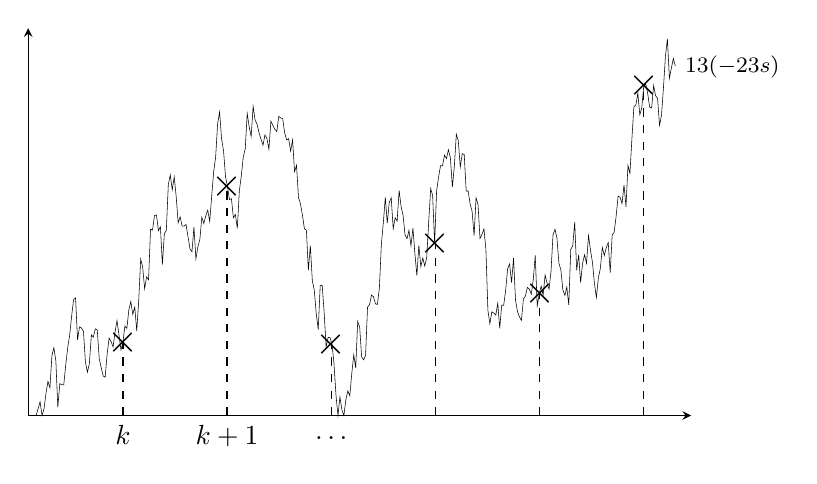
\begin{tikzpicture}
\pgfplotsset{ticks=none}

\begin{axis}[
xmin=0,
axis lines = middle,
xmax=4.2,
ymax = 3.5,
ymin  = 0,
width = 10cm,
height = 6.5cm,
clip=false
]

%%%%%%%%%%%%%%%%%%%%%%%%%%%%%%%%%%%%%%%%%%%%%%%%%%%%%%%%%%%%%%%%%%%%%%%%%%%%%%%%
% BROWNIAN MOTION
%%%%%%%%%%%%%%%%%%%%%%%%%%%%%%%%%%%%%%%%%%%%%%%%%%%%%%%%%%%%%%%%%%%%%%%%%%%%%%%%
\addplot [line width=0.2pt]coordinates{(0,0) (0.0125,0) (0.025,0) (0.0375,0) (0.05,0) (0.0625,0.06) (0.075,0.123) (0.0875,0) (0.1,0.06) (0.1125,0.2) (0.125,0.309) (0.1375,0.251) (0.15,0.539) (0.1625,0.613) (0.175,0.495) (0.1875,0.074) (0.2,0.288) (0.2125,0.279) (0.225,0.276) (0.2375,0.455) (0.25,0.611) (0.2625,0.724) (0.275,0.899) (0.2875,1.048) (0.3,1.062) (0.3125,0.684) (0.325,0.801) (0.3375,0.791) (0.35,0.761) (0.3625,0.482) (0.375,0.391) (0.3875,0.47) (0.4,0.728) (0.4125,0.709) (0.425,0.783) (0.4375,0.772) (0.45,0.511) (0.4625,0.432) (0.475,0.357) (0.4875,0.346) (0.5,0.555) (0.5125,0.7) (0.525,0.668) (0.5375,0.62) (0.55,0.753) (0.5625,0.858) (0.575,0.728) (0.5875,0.593) (0.6,0.662) (0.6125,0.808) (0.625,0.787) (0.6375,0.955) (0.65,1.03) (0.6625,0.914) (0.675,0.979) (0.6875,0.764) (0.7,1.036) (0.7125,1.413) (0.725,1.343) (0.7375,1.145) (0.75,1.253) (0.7625,1.227) (0.775,1.684) (0.7875,1.676) (0.8,1.807) (0.8125,1.813) (0.825,1.671) (0.8375,1.707) (0.85,1.364) (0.8625,1.643) (0.875,1.672) (0.8875,2.085) (0.9,2.175) (0.9125,2.04) (0.925,2.156) (0.9375,1.979) (0.95,1.741) (0.9625,1.796) (0.975,1.712) (0.9875,1.712) (1,1.726) (1.0125,1.614) (1.025,1.506) (1.0375,1.48) (1.05,1.704) (1.0625,1.415) (1.075,1.527) (1.0875,1.591) (1.1,1.793) (1.1125,1.735) (1.125,1.805) (1.1375,1.856) (1.15,1.753) (1.1625,1.983) (1.175,2.203) (1.1875,2.336) (1.2,2.638) (1.2125,2.744) (1.225,2.501) (1.2375,2.392) (1.25,2.16) (1.2625,2.07) (1.275,1.952) (1.2875,1.96) (1.3,1.787) (1.3125,1.817) (1.325,1.692) (1.3375,2.028) (1.35,2.164) (1.3625,2.337) (1.375,2.41) (1.3875,2.73) (1.4,2.609) (1.4125,2.521) (1.425,2.794) (1.4375,2.67) (1.45,2.631) (1.4625,2.556) (1.475,2.495) (1.4875,2.442) (1.5,2.536) (1.5125,2.502) (1.525,2.406) (1.5375,2.661) (1.55,2.621) (1.5625,2.586) (1.575,2.567) (1.5875,2.703) (1.6,2.689) (1.6125,2.682) (1.625,2.552) (1.6375,2.491) (1.65,2.502) (1.6625,2.39) (1.675,2.491) (1.6875,2.202) (1.7,2.261) (1.7125,1.969) (1.725,1.912) (1.7375,1.811) (1.75,1.687) (1.7625,1.676) (1.775,1.312) (1.7875,1.536) (1.8,1.22) (1.8125,1.132) (1.825,0.919) (1.8375,0.777) (1.85,1.173) (1.8625,1.177) (1.875,0.932) (1.8875,0.62) (1.9,0.706) (1.9125,0.703) (1.925,0.642) (1.9375,0.465) (1.95,0.183) (1.9625,0) (1.975,0.168) (1.9875,0.05) (2,0) (2.0125,0.142) (2.025,0.223) (2.0375,0.178) (2.05,0.379) (2.0625,0.548) (2.075,0.43) (2.0875,0.849) (2.1,0.801) (2.1125,0.53) (2.125,0.503) (2.1375,0.542) (2.15,0.981) (2.1625,1.001) (2.175,1.088) (2.1875,1.073) (2.2,1.009) (2.2125,1.003) (2.225,1.153) (2.2375,1.547) (2.25,1.742) (2.2625,1.972) (2.275,1.738) (2.2875,1.925) (2.3,1.967) (2.3125,1.688) (2.325,1.787) (2.3375,1.757) (2.35,2.035) (2.3625,1.889) (2.375,1.808) (2.3875,1.632) (2.4,1.598) (2.4125,1.674) (2.425,1.535) (2.4375,1.693) (2.45,1.463) (2.4625,1.264) (2.475,1.538) (2.4875,1.345) (2.5,1.423) (2.5125,1.351) (2.525,1.429) (2.5375,1.75) (2.55,2.051) (2.5625,1.988) (2.575,1.554) (2.5875,2.029) (2.6,2.156) (2.6125,2.258) (2.625,2.256) (2.6375,2.353) (2.65,2.322) (2.6625,2.402) (2.675,2.326) (2.6875,2.065) (2.7,2.253) (2.7125,2.542) (2.725,2.483) (2.7375,2.245) (2.75,2.367) (2.7625,2.358) (2.775,2.029) (2.7875,2.029) (2.8,1.91) (2.8125,1.845) (2.825,1.625) (2.8375,1.968) (2.85,1.905) (2.8625,1.6) (2.875,1.637) (2.8875,1.687) (2.9,1.5) (2.9125,0.951) (2.925,0.829) (2.9375,0.937) (2.95,0.926) (2.9625,0.907) (2.975,1.014) (2.9875,0.788) (3,0.997) (3.0125,0.996) (3.025,1.13) (3.0375,1.327) (3.05,1.369) (3.0625,1.202) (3.075,1.423) (3.0875,1.043) (3.1,0.94) (3.1125,0.891) (3.125,0.859) (3.1375,1.053) (3.15,1.079) (3.1625,1.157) (3.175,1.143) (3.1875,1.096) (3.2,1.229) (3.2125,1.446) (3.225,0.99) (3.2375,1.099) (3.25,1.17) (3.2625,1.089) (3.275,1.27) (3.2875,1.196) (3.3,1.142) (3.3125,1.305) (3.325,1.631) (3.3375,1.683) (3.35,1.603) (3.3625,1.377) (3.375,1.314) (3.3875,1.135) (3.4,1.086) (3.4125,1.161) (3.425,0.999) (3.4375,1.502) (3.45,1.532) (3.4625,1.747) (3.475,1.312) (3.4875,1.453) (3.5,1.202) (3.5125,1.377) (3.525,1.453) (3.5375,1.375) (3.55,1.627) (3.5625,1.494) (3.575,1.384) (3.5875,1.193) (3.6,1.066) (3.6125,1.246) (3.625,1.328) (3.6375,1.519) (3.65,1.445) (3.6625,1.517) (3.675,1.563) (3.6875,1.292) (3.7,1.63) (3.7125,1.656) (3.725,1.801) (3.7375,1.983) (3.75,1.973) (3.7625,1.915) (3.775,2.085) (3.7875,1.886) (3.8,2.26) (3.8125,2.188) (3.825,2.502) (3.8375,2.789) (3.85,2.805) (3.8625,2.913) (3.875,2.718) (3.8875,2.78) (3.9,2.978) (3.9125,2.997) (3.925,2.91) (3.9375,2.786) (3.95,2.779) (3.9625,2.982) (3.975,2.89) (3.9875,2.867) (4,2.621) (4.0125,2.715) (4.025,2.964) (4.0375,3.248) (4.05,3.403) (4.0625,3.048) (4.075,3.139) (4.0875,3.226) (4.1,3.159)
};


%%%%%%%%%%%%%%%%%%%%%%%%%%%%%%%%%%%%%%%%%%%%%%%%%%%%%%%%%%%%%%%%%%%%%%%%%%%%%%%%
% DASHED LINES
%%%%%%%%%%%%%%%%%%%%%%%%%%%%%%%%%%%%%%%%%%%%%%%%%%%%%%%%%%%%%%%%%%%%%%%%%%%%%%%%
\addplot [line width=0.5pt, dashed]coordinates{(0.6,0) (0.6,0.662)};
\addplot [line width=0.5pt, dashed]coordinates{(1.26,0) (1.26,2.07)};
\addplot [line width=0.5pt, dashed]coordinates{(1.92,0) (1.92,0.642)};
\addplot [line width=0.5pt, dashed]coordinates{(2.58,0) (2.58,1.554)};
\addplot [line width=0.5pt, dashed]coordinates{(3.24,0) (3.24,1.099)};
\addplot [line width=0.5pt, dashed]coordinates{(3.9,0) (3.9,2.978)};


%%%%%%%%%%%%%%%%%%%%%%%%%%%%%%%%%%%%%%%%%%%%%%%%%%%%%%%%%%%%%%%%%%%%%%%%%%%%%%%%
% LABELS
%%%%%%%%%%%%%%%%%%%%%%%%%%%%%%%%%%%%%%%%%%%%%%%%%%%%%%%%%%%%%%%%%%%%%%%%%%%%%%%%
\node at (axis cs:0.6,0)[anchor=north] {$k$};
\node at (axis cs:1.26,0)[anchor=north] {$k+1$};
\node at (axis cs:1.92,-0.1)[anchor=north] {$\dots$};
\node at (axis cs:2.58,-0.1)[anchor=north] {};
\node at (axis cs:3.24,0)[anchor=north] {};
\node at (axis cs:3.9,0)[anchor=north] {};


\node[font=\fontsize{15}{15}\selectfont] at (axis cs:0.6,0.662) {$\times$};
\node[font=\fontsize{15}{15}\selectfont] at (axis cs:1.26,2.07) {$\times$};
\node[font=\fontsize{15}{15}\selectfont] at (axis cs:1.92,0.642) {$\times$};
\node[font=\fontsize{15}{15}\selectfont] at (axis cs:2.58,1.554) {$\times$};
\node[font=\fontsize{15}{15}\selectfont] at (axis cs:3.24,1.099) {$\times$};
\node[font=\fontsize{15}{15}\selectfont] at (axis cs:3.9,2.978) {$\times$};

\node[font=\fontsize{8}{8}\selectfont] at (axis cs:4.1,3.15)[anchor = west] {$\n{1}{3}\BtX(\n{-2}{3}s)$};



\end{axis}

\end{tikzpicture} 
	\caption{The increments of $\Ndis$ are dependent on discrete steps of $\BtX$.} 
	\label{F: Mn}
\end{figure}

We will show that, if $||\rzntX - \WtX|| < \delta$, 
then $\Ndis(k) = \nntX(k)$ for all $k \leq \n{2}{3}T$ with high probability.
For this, we redefine both processes using a coupling argument.
At step $k$, let
\begin{equation} \label{E: def alpha beta}
\begin{aligned}
\alpha_k := \min(\zminzX(k), \n{1}{3}\BtX(\n{-2}{3}k)), \\
\beta_k := \max(\zminzX(k), \n{1}{3}\BtX(\n{-2}{3}k)),
\end{aligned}
\end{equation}
Now define random variables
\begin{equation} \label{E: def xi eta}
\begin{aligned}
\xi_k &\sim \Binom(\alpha_k, \p), \\
\eta_k &\sim \Binom(\beta_k - \alpha_k, \p).
\end{aligned}
\end{equation}
So $\xi_k + \eta_k \sim \Binom(\beta_k, \p)$.

\begin{figure}[ht]
	\centering
	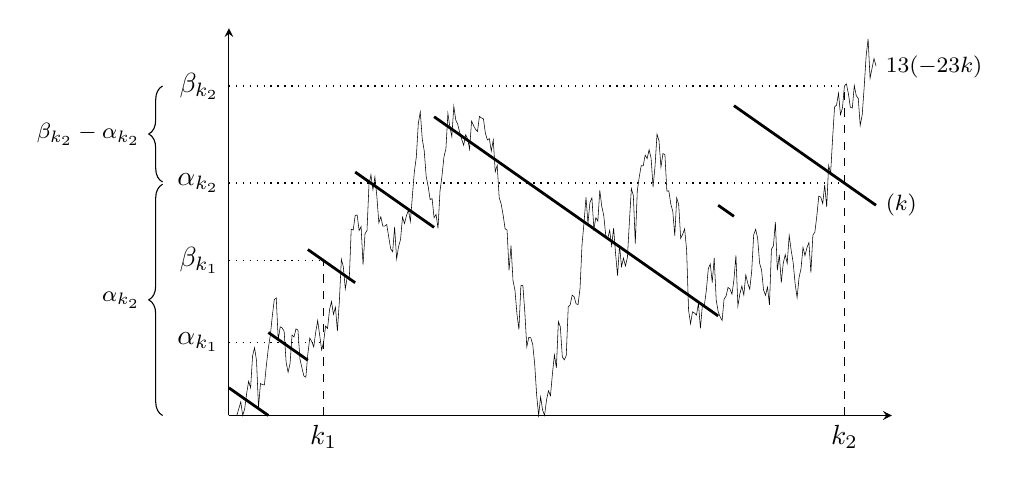
\begin{tikzpicture}
\pgfplotsset{ticks=none}

\begin{axis}[
xmin=0,
axis lines = middle,
xmax=4.2,
ymax = 3.5,
ymin  = 0,
width = 10cm,
height = 6.5cm,
clip=false
]


%%%%%%%%%%%%%%%%%%%%%%%%%%%%%%%%%%%%%%%%%%%%%%%%%%%%%%%%%%%%%%%%%%%%%%%%%%%%%%%%
% BF-WALK
%%%%%%%%%%%%%%%%%%%%%%%%%%%%%%%%%%%%%%%%%%%%%%%%%%%%%%%%%%%%%%%%%%%%%%%%%%%%%%%%
\addplot [line width=1.0pt]coordinates{(0,0.25) (0.25,0)};
\addplot [line width=1.0pt]coordinates{(0.25,0.75) (0.5,0.5)};
\addplot [line width=1.0pt]coordinates{(0.5,1.5) (0.8,1.2)};
\addplot [line width=1.0pt]coordinates{(0.8,2.2) (1,2)};
\addplot [line width=1.0pt]coordinates{(1,2) (1.3, 1.7)};
\addplot [line width=1.0pt]coordinates{(1.3, 2.7) (2,2)};
\addplot [line width=1.0pt]coordinates{(2,2) (3,1)};
\addplot [line width=1.0pt]coordinates{(3,1) (3.1, 0.9)};
\addplot [line width=1.0pt]coordinates{(3.1,1.9) (3.2,1.8)};
\addplot [line width=1.0pt]coordinates{(3.2,2.8) (4.1,1.9)};


%%%%%%%%%%%%%%%%%%%%%%%%%%%%%%%%%%%%%%%%%%%%%%%%%%%%%%%%%%%%%%%%%%%%%%%%%%%%%%%%
% BROWNIAN MOTION
%%%%%%%%%%%%%%%%%%%%%%%%%%%%%%%%%%%%%%%%%%%%%%%%%%%%%%%%%%%%%%%%%%%%%%%%%%%%%%%%
\addplot [line width=0.2pt]coordinates{(0,0) (0.0125,0) (0.025,0) (0.0375,0) (0.05,0) (0.0625,0.06) (0.075,0.123) (0.0875,0) (0.1,0.06) (0.1125,0.2) (0.125,0.309) (0.1375,0.251) (0.15,0.539) (0.1625,0.613) (0.175,0.495) (0.1875,0.074) (0.2,0.288) (0.2125,0.279) (0.225,0.276) (0.2375,0.455) (0.25,0.611) (0.2625,0.724) (0.275,0.899) (0.2875,1.048) (0.3,1.062) (0.3125,0.684) (0.325,0.801) (0.3375,0.791) (0.35,0.761) (0.3625,0.482) (0.375,0.391) (0.3875,0.47) (0.4,0.728) (0.4125,0.709) (0.425,0.783) (0.4375,0.772) (0.45,0.511) (0.4625,0.432) (0.475,0.357) (0.4875,0.346) (0.5,0.555) (0.5125,0.7) (0.525,0.668) (0.5375,0.62) (0.55,0.753) (0.5625,0.858) (0.575,0.728) (0.5875,0.593) (0.6,0.662) (0.6125,0.808) (0.625,0.787) (0.6375,0.955) (0.65,1.03) (0.6625,0.914) (0.675,0.979) (0.6875,0.764) (0.7,1.036) (0.7125,1.413) (0.725,1.343) (0.7375,1.145) (0.75,1.253) (0.7625,1.227) (0.775,1.684) (0.7875,1.676) (0.8,1.807) (0.8125,1.813) (0.825,1.671) (0.8375,1.707) (0.85,1.364) (0.8625,1.643) (0.875,1.672) (0.8875,2.085) (0.9,2.175) (0.9125,2.04) (0.925,2.156) (0.9375,1.979) (0.95,1.741) (0.9625,1.796) (0.975,1.712) (0.9875,1.712) (1,1.726) (1.0125,1.614) (1.025,1.506) (1.0375,1.48) (1.05,1.704) (1.0625,1.415) (1.075,1.527) (1.0875,1.591) (1.1,1.793) (1.1125,1.735) (1.125,1.805) (1.1375,1.856) (1.15,1.753) (1.1625,1.983) (1.175,2.203) (1.1875,2.336) (1.2,2.638) (1.2125,2.744) (1.225,2.501) (1.2375,2.392) (1.25,2.16) (1.2625,2.07) (1.275,1.952) (1.2875,1.96) (1.3,1.787) (1.3125,1.817) (1.325,1.692) (1.3375,2.028) (1.35,2.164) (1.3625,2.337) (1.375,2.41) (1.3875,2.73) (1.4,2.609) (1.4125,2.521) (1.425,2.794) (1.4375,2.67) (1.45,2.631) (1.4625,2.556) (1.475,2.495) (1.4875,2.442) (1.5,2.536) (1.5125,2.502) (1.525,2.406) (1.5375,2.661) (1.55,2.621) (1.5625,2.586) (1.575,2.567) (1.5875,2.703) (1.6,2.689) (1.6125,2.682) (1.625,2.552) (1.6375,2.491) (1.65,2.502) (1.6625,2.39) (1.675,2.491) (1.6875,2.202) (1.7,2.261) (1.7125,1.969) (1.725,1.912) (1.7375,1.811) (1.75,1.687) (1.7625,1.676) (1.775,1.312) (1.7875,1.536) (1.8,1.22) (1.8125,1.132) (1.825,0.919) (1.8375,0.777) (1.85,1.173) (1.8625,1.177) (1.875,0.932) (1.8875,0.62) (1.9,0.706) (1.9125,0.703) (1.925,0.642) (1.9375,0.465) (1.95,0.183) (1.9625,0) (1.975,0.168) (1.9875,0.05) (2,0) (2.0125,0.142) (2.025,0.223) (2.0375,0.178) (2.05,0.379) (2.0625,0.548) (2.075,0.43) (2.0875,0.849) (2.1,0.801) (2.1125,0.53) (2.125,0.503) (2.1375,0.542) (2.15,0.981) (2.1625,1.001) (2.175,1.088) (2.1875,1.073) (2.2,1.009) (2.2125,1.003) (2.225,1.153) (2.2375,1.547) (2.25,1.742) (2.2625,1.972) (2.275,1.738) (2.2875,1.925) (2.3,1.967) (2.3125,1.688) (2.325,1.787) (2.3375,1.757) (2.35,2.035) (2.3625,1.889) (2.375,1.808) (2.3875,1.632) (2.4,1.598) (2.4125,1.674) (2.425,1.535) (2.4375,1.693) (2.45,1.463) (2.4625,1.264) (2.475,1.538) (2.4875,1.345) (2.5,1.423) (2.5125,1.351) (2.525,1.429) (2.5375,1.75) (2.55,2.051) (2.5625,1.988) (2.575,1.554) (2.5875,2.029) (2.6,2.156) (2.6125,2.258) (2.625,2.256) (2.6375,2.353) (2.65,2.322) (2.6625,2.402) (2.675,2.326) (2.6875,2.065) (2.7,2.253) (2.7125,2.542) (2.725,2.483) (2.7375,2.245) (2.75,2.367) (2.7625,2.358) (2.775,2.029) (2.7875,2.029) (2.8,1.91) (2.8125,1.845) (2.825,1.625) (2.8375,1.968) (2.85,1.905) (2.8625,1.6) (2.875,1.637) (2.8875,1.687) (2.9,1.5) (2.9125,0.951) (2.925,0.829) (2.9375,0.937) (2.95,0.926) (2.9625,0.907) (2.975,1.014) (2.9875,0.788) (3,0.997) (3.0125,0.996) (3.025,1.13) (3.0375,1.327) (3.05,1.369) (3.0625,1.202) (3.075,1.423) (3.0875,1.043) (3.1,0.94) (3.1125,0.891) (3.125,0.859) (3.1375,1.053) (3.15,1.079) (3.1625,1.157) (3.175,1.143) (3.1875,1.096) (3.2,1.229) (3.2125,1.446) (3.225,0.99) (3.2375,1.099) (3.25,1.17) (3.2625,1.089) (3.275,1.27) (3.2875,1.196) (3.3,1.142) (3.3125,1.305) (3.325,1.631) (3.3375,1.683) (3.35,1.603) (3.3625,1.377) (3.375,1.314) (3.3875,1.135) (3.4,1.086) (3.4125,1.161) (3.425,0.999) (3.4375,1.502) (3.45,1.532) (3.4625,1.747) (3.475,1.312) (3.4875,1.453) (3.5,1.202) (3.5125,1.377) (3.525,1.453) (3.5375,1.375) (3.55,1.627) (3.5625,1.494) (3.575,1.384) (3.5875,1.193) (3.6,1.066) (3.6125,1.246) (3.625,1.328) (3.6375,1.519) (3.65,1.445) (3.6625,1.517) (3.675,1.563) (3.6875,1.292) (3.7,1.63) (3.7125,1.656) (3.725,1.801) (3.7375,1.983) (3.75,1.973) (3.7625,1.915) (3.775,2.085) (3.7875,1.886) (3.8,2.26) (3.8125,2.188) (3.825,2.502) (3.8375,2.789) (3.85,2.805) (3.8625,2.913) (3.875,2.718) (3.8875,2.78) (3.9,2.978) (3.9125,2.997) (3.925,2.91) (3.9375,2.786) (3.95,2.779) (3.9625,2.982) (3.975,2.89) (3.9875,2.867) (4,2.621) (4.0125,2.715) (4.025,2.964) (4.0375,3.248) (4.05,3.403) (4.0625,3.048) (4.075,3.139) (4.0875,3.226) (4.1,3.159)
};


%%%%%%%%%%%%%%%%%%%%%%%%%%%%%%%%%%%%%%%%%%%%%%%%%%%%%%%%%%%%%%%%%%%%%%%%%%%%%%%%
% DOTTED LINES
%%%%%%%%%%%%%%%%%%%%%%%%%%%%%%%%%%%%%%%%%%%%%%%%%%%%%%%%%%%%%%%%%%%%%%%%%%%%%%%%
\addplot [line width=0.5pt, dotted]coordinates{(0,2.978) (3.9,2.978)};
\addplot [line width=0.5pt, dotted]coordinates{(0,2.1) (3.9,2.1)};
\addplot [line width=0.5pt, dashed]coordinates{(3.9,0) (3.9,2.978)};

\addplot [line width=0.5pt, dotted]coordinates{(0,1.4) (0.6,1.4)};
\addplot [line width=0.5pt, dotted]coordinates{(0,0.662) (0.6,0.662)};
\addplot [line width=0.5pt, dashed]coordinates{(0.6,0) (0.6,1.4)};



%%%%%%%%%%%%%%%%%%%%%%%%%%%%%%%%%%%%%%%%%%%%%%%%%%%%%%%%%%%%%%%%%%%%%%%%%%%%%%%%
% LABELS
%%%%%%%%%%%%%%%%%%%%%%%%%%%%%%%%%%%%%%%%%%%%%%%%%%%%%%%%%%%%%%%%%%%%%%%%%%%%%%%%
\node at (axis cs:0.6,0)[anchor=north] {$k_1$};
\node at (axis cs:3.9,0)[anchor=north] {$k_2$};

\node[font=\fontsize{8}{8}\selectfont] at (axis cs:4.1,1.9)[anchor = west] {$\zminz(k)$};
\node[font=\fontsize{8}{8}\selectfont] at (axis cs:4.1,3.15)[anchor = west] {$\n{1}{3}\Bt(\n{-2}{3}k)$};

\node at (axis cs:0,2.1)[anchor = east] {$\alpha_{k_2}$};
\node at (axis cs:0,0.662)[anchor = east] {$\alpha_{k_1}$};
\node at (axis cs:0,2.978)[anchor = east] {$\beta_{k_2}$};
\node at (axis cs:0,1.4)[anchor = east] {$\beta_{k_1}$};


%%%%%%%%%%%%%%%%%%%%%%%%%%%%%%%%%%%%%%%%%%%%%%%%%%%%%%%%%%%%%%%%%%%%%%%%%%%%%%%%
% BRACES
%%%%%%%%%%%%%%%%%%%%%%%%%%%%%%%%%%%%%%%%%%%%%%%%%%%%%%%%%%%%%%%%%%%%%%%%%%%%%%%%
\draw [decorate,decoration={brace,amplitude=5pt,raise=4pt},yshift=0pt]
(axis cs: -0.35,0) -- (axis cs: -0.35,2.09) node [black,midway,xshift=-0.3cm, anchor = east] {\footnotesize
	$\alpha_{k_2}$};
\draw [decorate,decoration={brace,amplitude=5pt,raise=4pt},yshift=0pt]
(axis cs: -0.35,2.11) -- (axis cs: -0.35,2.978) node [black,midway,xshift=-0.3cm, anchor = east] {\footnotesize
$\beta_{k_2} - \alpha_{k_2}$};

\end{axis}

\end{tikzpicture} 
	\caption{The upscaled reflected Brownian motion and the reflected breadth-first walk define $\alpha_k$ and $\beta_k$.} 
	\label{F: BM BF-walk}
\end{figure}

Consider the two possibilities at time $k$:
Either $\zminzX(k) \leq \n{1}{3}\BtX(\n{-2}{3}k)$,
then $\alpha_k = \zminzX(k)$ and $\beta_k = \n{1}{3}\BtX(\n{-2}{3}k)$, 
so 
\begin{equation}
\begin{aligned}
\xi_k &=_d \nntX(k) - \nntX(k-1), \\
\xi_k + \eta_k &=_d \Ndis(k) - \Ndis(k-1).
\end{aligned}
\end{equation}
Or $\zminzX(k) > \n{1}{3}\BtX(\n{-2}{3}k)$,
then $\alpha_k = \n{1}{3}\BtX(\n{-2}{3}k)$ and $\beta_k = \zminzX(k)$, 
so
\begin{equation}
\begin{aligned}
\xi_k &=_d \Ndis(k) - \Ndis(k-1), \\
\xi_k + \eta_k &=_d \nntX(k) - \nntX(k-1).
\end{aligned}
\end{equation}

This way, we can define $\nntX$ and $\Ndis$ by
\begin{equation}
\nntX(k) - \nntX(k-1) = 
\begin{cases}
\xi_k & \text{if} \enspace \zminzX(k) \leq \n{1}{3}\BtX(\n{-2}{3}k), \\
\xi_k + \eta_k &\text{else}
\end{cases}
\end{equation}
and
\begin{equation}
\Ndis(k) - \Ndis(k-1) = 
\begin{cases}
\xi_k + \eta_k & \text{if} \enspace \zminzX(k) \leq \n{1}{3}\BtX(\n{-2}{3}k), \\
\xi_k &\text{else}.
\end{cases}
\end{equation}
By \eqref{E: def alpha beta} and \eqref{E: def xi eta},
these definitions maintain
\begin{equation*}
\begin{aligned}
\nntX(k) - \nntX(k-1) &\sim \Binom(\zminzX(k), \p), \\
\Ndis(k) - \Ndis(k-1) &\sim \Binom(\n{1}{3} \BtX(\n{-2}{3}k), \p).
\end{aligned}
\end{equation*}
We see that, no matter the relation of $\zminzX(k)$ and $\n{1}{3}\BtX(\n{-2}{3}k)$, 
the increments of the processes differ only by the random variable $\eta_k$.

Conditioning on $||\rzntX - \WtX|| < \delta$, for $\Ndis(k) \neq \nntX(k)$ to hold for some $k$,
there has to have been a step in which the increments of both processes were different.
We evaluate
\begin{equation} \label{E: Prob eta not 0}
\begin{aligned}
&\Prob(\exists k\leq \n{2}{3}T: \Ndis(k) \neq \nntX(k) \cond \Event{\delta}) \\
&\quad \leq \sum_{k=1}^{\n{2}{3}T} \Prob( \Ndis(k) - \Ndis(k-1) \neq \nntX(k) - \nntX(k-1) \cond \Event{\delta}) \\
&\quad \leq \sum_{k=1}^{\n{2}{3}T} \Prob( \eta_k \neq 0 \cond \Event{\delta}) \\
&\quad \leq \n{2}{3}T \max_{k \leq \n{2}{3}T} \Prob(\eta_k \neq 0 \cond \Event{\delta}).
\end{aligned}
\end{equation}

Since $||\znt - \WtX|| < \delta$, we know $\beta_k - \alpha_k < \delta \n{1}{3}$. Therefore
$\eta_k \leq_{\text{st.}} \zeta \sim \Binom(\delta\n{1}{3}, \p)$ for all $k \leq \n{2}{3}T$.

Using Markov's inequality gives
\begin{equation}
\Prob( \eta_k \neq 0 \cond \Event{\delta} ) \leq \Prob( \zeta_k \geq 1 ) \leq \Exp{\zeta_k} = \delta\n{1}{3}\p,
\end{equation}
and substituting in \eqref{E: Prob eta not 0} we obtain
\begin{equation}
\begin{aligned}
&\Prob(\exists k\leq \n{2}{3}T: \Ndis(k) \neq \nntX(k) \cond \Event{\delta}) \\
&\quad \leq \n{2}{3}T \max_{k \leq \n{2}{3}T} \Prob( \eta_k \neq 0 \cond \Event{\delta} ) \\
&\quad \leq \n{2}{3}T\delta\n{1}{3}\p \\
&\quad \leq n \p T \delta \\
&\quad \leq 2T\delta 
\end{aligned}
\end{equation}
for large $n$.

We now define $\rNdisX(s) = \n{-1}{3} \Ndis(\n{2}{3}s)$ and continue the estimation from \eqref{E: Estimation step 3},
which yields
\begin{equation} \label{E: Estimation step 4}
\begin{aligned}
\Exp{f(\rzntX, \nntX)} 
&\leq \Exp{f(\WtX, \nntX) \cond \Event{C}, \Event{\delta}} \Prob(\Event{C}) \Prob(\Event{\delta}) + \epsilon + 2M\epsilon   \\
&\leq \Exp{f(\WtX, \rNdisX) \cond \Event{C}, \Event{\delta}} \Prob(\Event{C}) \Prob(\Event{\delta}) + 2\delta T M + \epsilon  + 2M\epsilon \\
&\leq \Exp{f(\WtX, \rNdisX)} + 2\delta T M + \epsilon  + 2M\epsilon.
\end{aligned}
\end{equation}
This inequality holds for all bounded, continuous functions $f$. 
Therefore it holds for $-f$ as well, which implies
\begin{equation}
\begin{aligned}
\Exp{-f(\rzntX, \nntX)} &\leq \Exp{-f(\WtX, \rNdisX) }+ 2\delta T M  + \epsilon + 2M\epsilon \\
\iff  \Exp{f(\rzntX, \nntX)} &\geq \Exp{f(\WtX, \rNdisX) } - 2\delta T M  - \epsilon - 2M\epsilon,
\end{aligned}
\end{equation}
and therefore
\begin{equation} \label{E: Equality of Expectations}
	|\Exp{f(\rzntX, \nntX)} - \Exp{f(\WtX, \rNdisX)} | \leq 2\delta T M + \epsilon  + 2M\epsilon.
\end{equation}
\end{proofpart}



%%%%%%%%%%%%%%%%%%%%%%%%%%%%%%%%%%%%%%%%%%%%%%%%%%%%%%%%%%%%
% Proofpart 4: M ->_d N
%%%%%%%%%%%%%%%%%%%%%%%%%%%%%%%%%%%%%%%%%%%%%%%%%%%%%%%%%%%%
\begin{proofpart}
We now show that for any realization of $\WtX$ we have $\rNdisX \rightarrow_d \NtX$.
Fix $\WtX = \WtX(\omega)$ and therefore $\BtX = \BtX(\omega)$.
Since $\nntX$ is tight and $\nntX$ is equal to $\Ndis$ with high probability,
$\Ndis$ and $\rNdisX$ are tight and it suffices proving convergence in finite dimensional distributions,
in this case for all $0 \leq s_1 < s_2 < \dots < s_l \leq T$:
\begin{equation} \label{E: convergence fdd}
\begin{aligned}
&\Prob( \rNdisX(s_1) = k_1, \dots, \rNdisX(s_l) = k_l ) \\
&\quad \xrightarrow{n \rightarrow \infty}  \Prob( \NtX(s_1) = k_1, \dots, \NtX(s_l) = k_l ).
\end{aligned}
\end{equation}

Recall that $\NtX$ is a Poisson point process, continuous on $\Real$ with rate $\BtX$,
thus the increments of $\NtX$ are independent and for all $a<b$: 
\begin{equation}
\NtX(b) - \NtX(a) \sim \Poisson( \int_{a}^{b} \BtX(s)ds).
\end{equation}
In contrast, $\Ndis$ is a discrete process whose increments are defined by $\BtX$ at integer times, 
that is for all $k \leq \n{2}{3}T$: 
\begin{equation} \label{E: increments Ndis 2}
\Ndis(k) - \Ndis(k-1) \sim \Binom(\n{1}{3}\BtX(\n{-2}{3}k), \p)
\end{equation}
We can evaluate the distribution of the increments of $\rNdisX$ by
\begin{equation}
\rNdisX(s) - \rNdisX(s-1) = \n{-1}{3}( \Ndis(\n{2}{3}s) - \Ndis(\n{2}{3}(s-1))
\end{equation}
for $s \leq T$.
Between times $\n{2}{3}(s-1)$ and $\n{2}{3}s$, there are multiple integer steps,
the increment in each step as defined in \eqref{E: increments Ndis 2}. 
Therefore
\begin{equation}
\rNdisX(s_j) - \rNdisX(s_{j-1}) \sim \n{-1}{3} \sum_{i=\n{2}{3}s_{j-1}+1}^{\n{2}{3}s_j} \Binom( \n{1}{3}\BtX(\n{-2}{3}i), \p ).
\end{equation}
Since the increments are independent, we can move the sum inside the argument of the Binomial distribution.
Let us define 
\begin{equation*}
R_{n,j} := \sum_{i=\n{2}{3}s_{j-1}+1}^{\n{2}{3}s_j}\n{1}{3}\BtX(\n{-2}{3}i)
\end{equation*}
and compute the probability in \eqref{E: convergence fdd} as
\begin{equation} \label{E: distribution Ndis}
\begin{aligned}
&\Prob(\rNdisX(s_1) = k_1, \dots, \rNdisX(s_l) = k_l) \\
&\quad = \Prob( \rNdisX(s_j) - \rNdisX(s_{j-1}) = k_j - k_{j-1}, \enspace \forall j=2,\dots,l ) \\
&\quad = \prod_{j=2}^{l} \Prob( \n{1}{3}\rNdisX(s_j) - \n{1}{3}\rNdisX(s_{j-1}) = \n{1}{3}(k_j - k_{j-1})) \\
&\quad = \prod_{j=2}^{l} \Prob( Y_{n,j} = \n{1}{3}(k_j - k_{j-1}) ),
\end{aligned}
\end{equation}
where $Y_{n,j} \sim \Binom(R_{n,j}, \p)$.
Note that $Y_{n,j} =_d \sum_{k=1}^{R_{n,j}} \xi_k$, with $\xi_k \sim \Bern(\p)$.

In the next step we use the Poisson limit theorem, see for example \cite[Theorem 3.7, p.79]{Klenke.2006},
which states that for a series of binomially distributed random variables $X_k \sim \Binom(N_k, p_k)$
with $\Exp{X_k} = N_k p_k \rightarrow \lambda \in \Real$ as $k \rightarrow \infty$,
the convergence 
\begin{equation}
	X_k \rightarrow_d \Poisson(\lambda)
\end{equation}
holds as $k \rightarrow \infty$.
To apply this theorem, we calculate the expected value of $Y_{n,j}$:
\begin{align*}
\Exp{Y_{n,j}} 
&= R_{n,j} \p \\
&= \frac{1}{n} R_{n,j} + \BigO{\n{-1}{3}}\\
&= \frac{1}{n} \sum_{i=\n{2}{3}s_{j-1}+1}^{\n{2}{3}s_j}\n{1}{3}\BtX(\n{-2}{3}i) + \BigO{\n{-1}{3}}\\
&= \sum_{i=\n{2}{3}s_{j-1}+1}^{\n{2}{3}s_j}\n{-2}{3}\BtX(\n{-2}{3}i) + \BigO{\n{-1}{3}}
\end{align*}
This sum represents a partition of the interval $[s_{j-1}, s_j]$ into $\n{2}{3}(s_j - s_{j-1})$ subintervals, each of length $\n{-2}{3}$.
Since $\n{-2}{3}i$ is an element of its corresponding subinterval, 
we are dealing with a Riemann sum over the continuous function $\BtX$.
Since $\BtX$ is bounded almost surely on the compact interval $[s_{j-1}, s_j]$,
the sum converges to an integral and
\begin{equation}
\Exp{Y_{n,j}} \rightarrow \int_{s_{j-1}}^{s_j} \BtX(u)du.
\end{equation}
Now applying the Poisson limit theorem yields
\begin{equation} \label{E: convergence dist Yj}
Y_{n,j} \rightarrow_d \Poisson( \int_{s_{j-1}}^{s_j} \BtX(u)du ) =_d \NtX(s_j) - \NtX(s_{j-1}),
\end{equation}
and, applying this convergence in \eqref{E: distribution Ndis}, we arrive at
\begin{equation*}
\begin{aligned}
&\Prob(\rNdisX(s_1) = k_1, \dots, \rNdisX(s_l) = k_l) \\
&\quad = \prod_{j=2}^{l} \Prob( Y_{n,j} = \n{1}{3}(k_j - k_{j-1}) ) \\
&\enspace \rightarrow \prod_{j=2}^{l} \Prob( \NtX(s_j) - \NtX(s_{j-1}) = \n{1}{3}(k_j - k_{j-1}) ) \\
&\quad = \Prob(\NtX(s_1) = k_1, \dots, \NtX(s_l) = k_l).
\end{aligned}
\end{equation*}

For any fixed $\WtX(\omega)$ we therefore have $\rNdisX \rightarrow_d \NtX$.
Since $f(\WtX, \cdot)$ is abounded continuous function this implies
\begin{equation}
	\Exp{f(\WtX(\omega), \rNdisX)} \rightarrow \Exp{f(\WtX(\omega), \NtX)}
\end{equation}
or
\begin{equation}
	\Exp{f(\WtX(\omega), \rNdisX) \cond \WtX(\omega)} \rightarrow_{a.s.} \Exp{f(\WtX(\omega), \NtX)\cond \WtX(\omega)}.
\end{equation}
by the boundedness of $f$ we can apply the dominated convergence theorem which gives
\begin{equation}
	\begin{aligned}
	\Exp{f(\WtX, \NtX)}
	&= \Exp{ \Exp{f(\WtX(\omega), \NtX) \cond \WtX(\omega)} } \\
	&= \Exp{ \lim_{n->\infty} \Exp{f(\WtX(\omega), \rNdisX) \cond \WtX(\omega)} } \\
	&= \lim_{n->\infty} \Exp{ \Exp{f(\WtX(\omega), \rNdisX) \cond \WtX(\omega)} } \\
	&= \lim_{n->\infty} \Exp{ f(\WtX, \rNdisX) }.
	\end{aligned}
\end{equation}
Finally, the closeness of $\Exp{ f(\WtX, \rNdisX) }$ and $\Exp{f(\rzntX, \nntX)}$ in \eqref{E: Equality of Expectations} implies
\begin{equation}
	\Exp{f(\rzntX, \nntX)} \rightarrow \Exp{f(\WtX, \NtX)}
\end{equation}
which completes the proof.
\end{proofpart}
\end{proof}


We can now assure ourselves that the overestimated probability \eqref{E: rate Nnt} is asymptotically negligible.
Assume the chance that any vertex encounters two or more surplus edges is non-zero and does not converge to zero as $n \rightarrow \infty$.
If a vertex connects by multiple excess edges, the process $\nnt$ makes two or more jumps during the time-interval of length $1$.
The rescaling \eqref{E: rescale Nnt} compresses the time axis until, in the limit process $\Nt$, 
any distance in an interval of original length $1$ will be reduced to a single point.
Consequently there would be a non-zero chance that the counting process has multiple coincident points.
But since $\int_{\{x\}} \Bt(s)ds = 0$ for all $x \in \Rplus$, 
$\Nt$ is simple and the probability of multiple coincident points occurring is $0$.
We conclude that the probability of a vertex having multiple surplus edges must tend to zero.


